\documentclass[12pt]{article}
\usepackage[letterpaper]{geometry}
\usepackage{fontenc}
\usepackage{graphicx}
\usepackage[spanish,es-tabla]{babel}
\usepackage{amssymb}
\usepackage{amsmath}
\usepackage{graphicx}
\usepackage{subcaption}
\title{Pathfinding}
\author{Padilla Herrera Carlos Ignacio}
\date{}

\begin{document}

\maketitle

\begin{abstract}
Resumen del trabajo
\end{abstract}

\section{Introducción}
Este código es una implementación de un algoritmo de pathfinding, utilizando el
algoritmo de Dijkstra, para encontrar el camino más corto entre dos puntos en un
mapa. El mapa se representa como una matriz de 20x20, en la cual se generan aleatoriamente
obstáculos. Se establecen las posiciones iniciales y finales de dos agentes, A1 y A2, y se ejecuta
el algoritmo para encontrar el camino más corto entre cada uno de los agentes y su destino. Además
se muestra una representación gráfica del mapa, donde se pueden visualizar los obstáculos, los agentes
y los caminos encontrados.

\section{Metodología}
\subsection{Algoritmos de solución}
Este código utiliza el algoritmo de Dijkstra para encontrar el camino mínimo en un mapa
representado por una matriz de 20x20. El algoritmo comienza en una posición inicial especificada y
utiliza una cola de prioridad para explorar cada uno de los vecinos del nodo actual, asignando una
distancia a cada uno de ellos y actualizando la distancia si se encuentra un camino más corto.
Además, se almacena el camino desde el nodo inicial hasta cada uno de los nodos visitados. En este
caso se esta utilizando dos agentes A1 y A2, que tienen posiciones iniciales y finales diferentes,
el algoritmo busca el camino mínimo para cada uno de los agentes.

\subsection{Programación de algoritmos}
El algoritmo de Dijkstra es un algoritmo de búsqueda de camino que se utilzia para encontrar el camino 
más corto entre dos puntos en un grafo o mapa. En esta implementación se utiliza una matriz para 
representar el mapa y se utiliza la librería \textit{heapq} para crear una cola de prioridad donde se 
almacenan los nodos a explorar. La distancia entre el nodo inicial y cada uno de los nodos visitados 
es almacenada en un diccionario \textit{visitados}. También se crea un diccionario \textit{camino} que almacena el 
camino desde el nodo inicial hasta cada uno de los nodos visitados.
El algoritmo comienza agregando el nodo inicial a la cola de prioridad con una distancia de 0. Luego, 
mientras la cola no esté vacía, se extrae el primer elemento de la cola (el nodo con la distancia más 
corta) y se marca como visitado.
Se recorren sus vecinos, y se actualiza la distancia y el camino si se encuentra 
un camino más corto.
Finalmente, el algoritmo devuelve el camino más corto entre el nodo inicial y 
el destino, que se puede encontrar en el diccionario \textit{camino}.

\section{Pruebas}
\subsection{Pruebas para un agente con un inicio y un destino}
En esta sección se describen y presentan los resultados de las pruebas realizadas con un agente y un inicio y destino determinado.

\subsection{Pruebas para dos agentes con el mismo destino}
En esta sección se describen y presentan los resultados de las pruebas realizadas con dos agentes y el mismo destino.
\begin{figure}
    \centering
    \begin{subfigure}{.5\textwidth}
      \centering
      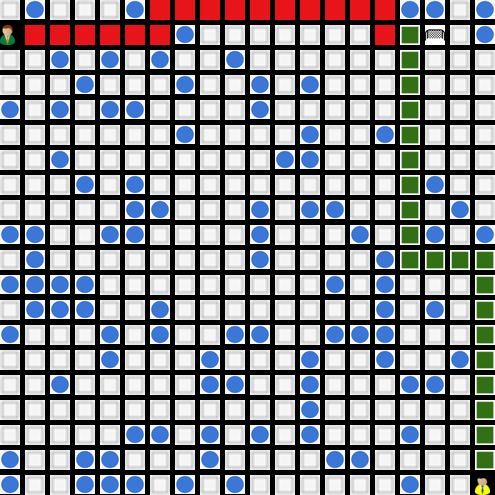
\includegraphics[width=.4\linewidth]{agente-mismo-destino.png}
      \caption{Agentes con el mismo destino en interfaz gráfica con pygame.}
      
    \end{subfigure}%
    \begin{subfigure}{.5\textwidth}
      \centering
      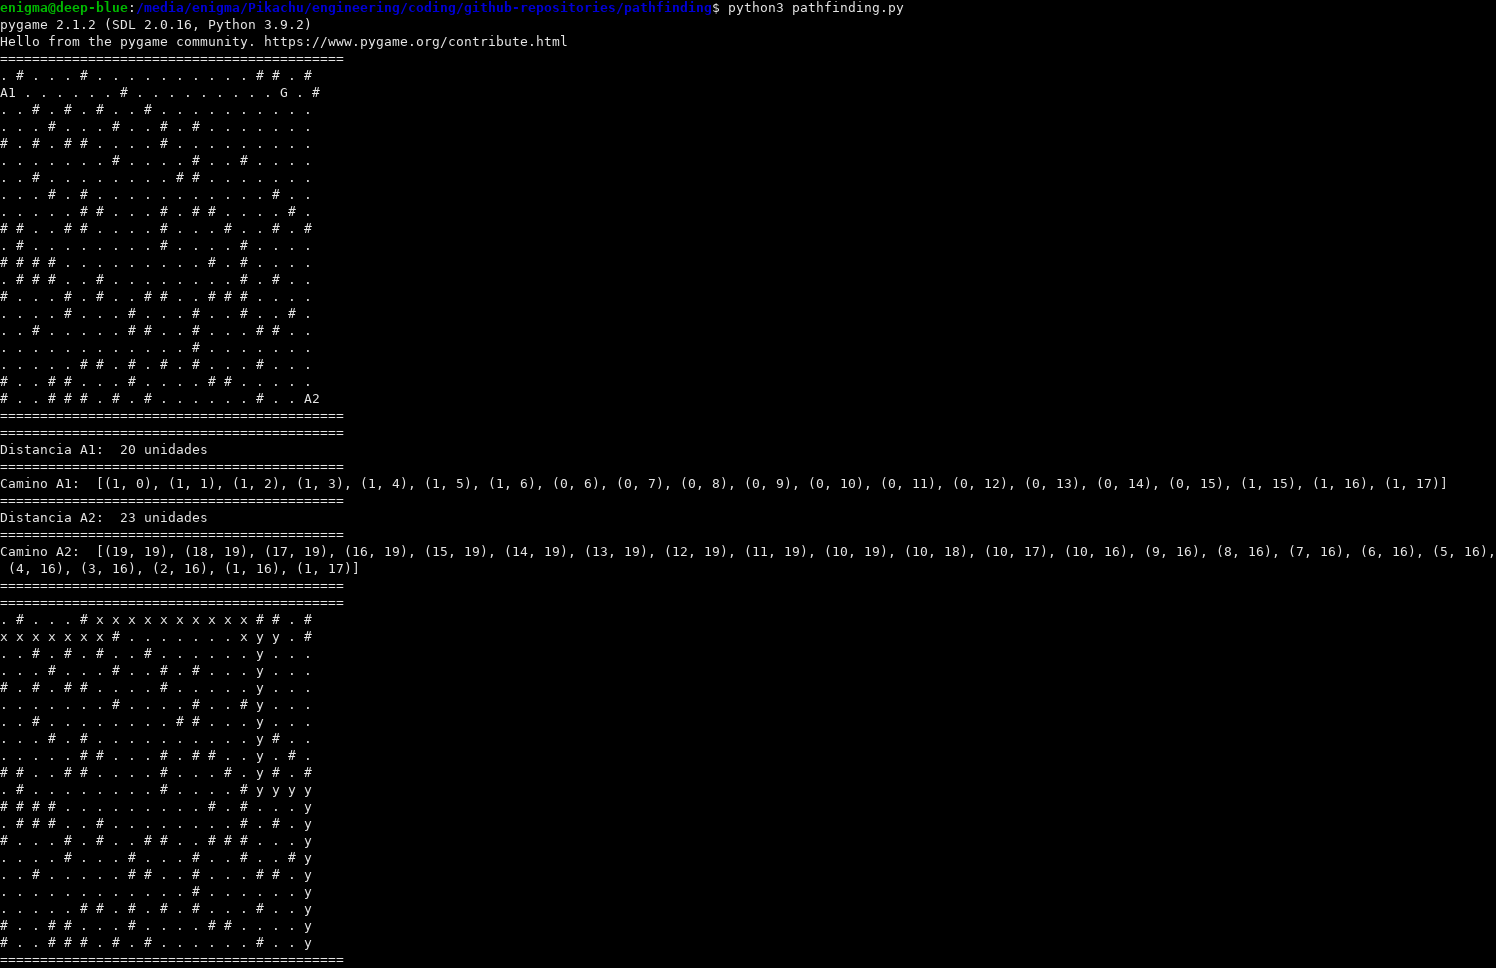
\includegraphics[width=.4\linewidth]{agente-mismo-destino-2.png}
      \caption{Imagen 2}
      
    \end{subfigure}
    \caption{Agentes con el mismo destino, la salida en terminal de consola.}
    
    \end{figure}

\subsection{Pruebas para dos agentes con destinos diferentes}
En esta sección se describen y presentan los resultados de las pruebas realizadas con dos agentes y destinos diferentes.

\subsection{Pruebas comparativas con dos tipos de algoritmos}
En esta sección se describen y presentan los resultados de las pruebas comparativas realizadas entre dos tipos de algoritmos.

\section{Resultados}
En esta sección se presentan los resultados obtenidos en las pruebas descritas en la sección anterior.

\section{Conclusiones}
En esta sección se describen las conclusiones a las que se llegó tras la realización del trabajo.

\section{Referencias bibliográficas}
En esta sección se listan las referencias bibliográficas utilizadas en el trabajo.

\end{document}
